\documentclass[12pt]{article}
\usepackage{graphicx}
\usepackage{caption}
\usepackage{float}
\usepackage[a4paper,margin=1in,footskip=0.25in]{geometry}
\usepackage{pdfpages}
\usepackage{setspace}
\doublespace
% \usepackage[english]{babel}
% \usepackage[style=ieee,backend=biber]{biblatex}
% \addbibresource{lab.bib}
\usepackage{hyperref}
\hypersetup{
    colorlinks,
    citecolor=black,
    filecolor=black,
    linkcolor=black,
    urlcolor=black
}

\begin{document}

\title{Polyopticon SDS}
\author{Jon Bakies \and Mitchell Dunn} 

\maketitle
\newpage

%\tableofcontents
%\newpage

\section{Summary Of Proposal}
\paragraph{}
Polyopticon is a portable presentation tool that consists of a projector, camera, Raspberry Pi, and an infrared(IR) LED drawing tool.
The camera, pointed at the projected surface, captures the user's pen strokes with image recognition of the IR LED.
Originally the Raspberry Pi was intended to project and handle all of the image processing, but after testing it was determined that the Raspberry Pi could not handle such a demanding task.
Instead of performing the image recognition on the Raspberry Pi, the Pi streams the video to the user's computer to be processed.

\section{Design}
\subsection{Dataflow}
\begin{figure}[ht!]
\centering
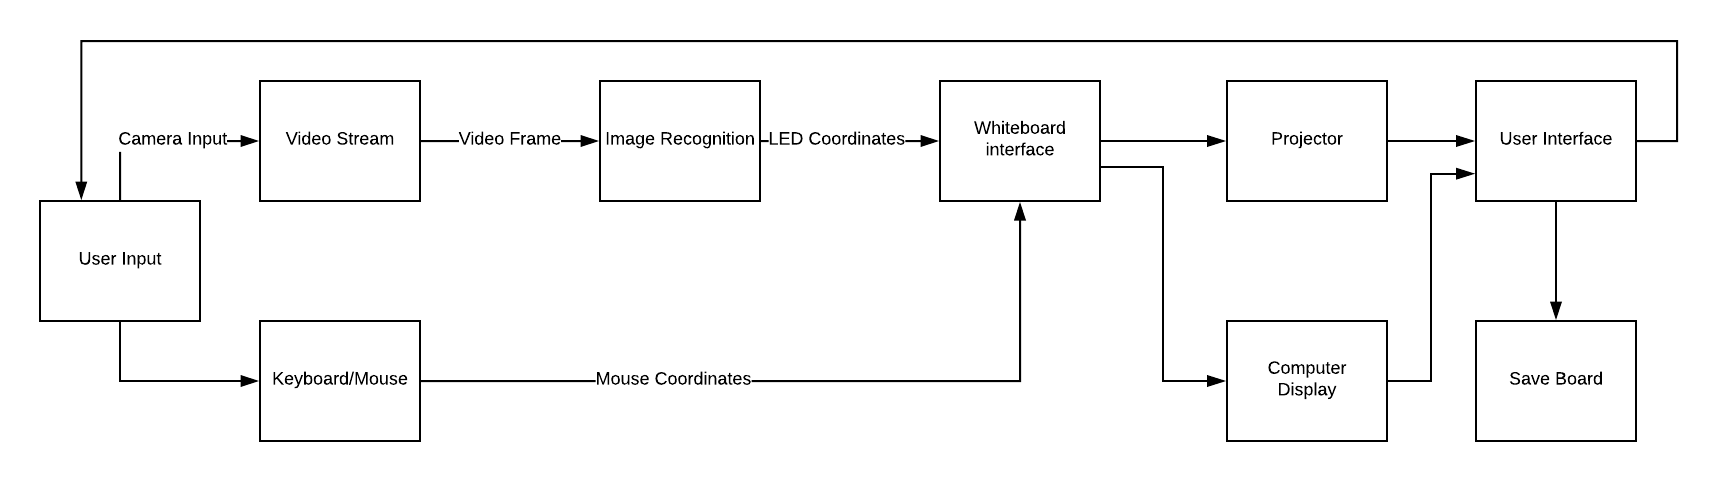
\includegraphics[width=\textwidth, height=\textheight, keepaspectratio]{Dataflow.png}
\end{figure}
\paragraph{}
The user can input data from the projected user interface via the IR LED and the camera, or from their personal computer where they can directly interact with the whiteboard interface.
The video from the camera is streamed to the user's computer and passed through OpenCV frame by frame to search for the LED.  
Once the LED is found, the coordinates are sent to the whiteboard interface to display pen strokes.
The whiteboard interface is projected and displayed on the user's computer and makes up the user interface.
\subsection{Image Recognition}
\begin{figure}[H]
\centering
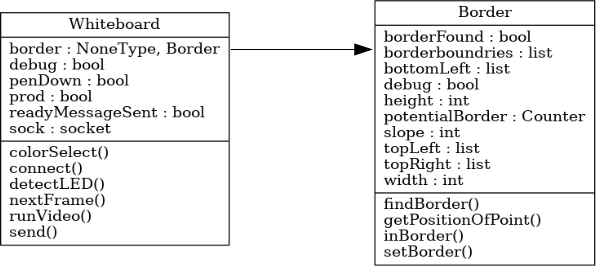
\includegraphics[scale=.5]{classdiagram.png}
\end{figure}
\paragraph{}
The Image Recognition part of Polyopticon is written in python and consists of two classes.
The Whiteboard class locates the LED in an image using OpenCV and sends the coordinates to the whiteboard interface through a socket.
The Border class stores information about the border of the drawable space, and contains methods to determine if coordinates are within the border.
\subsection{User interface} 
\begin{figure}[H]
\centering
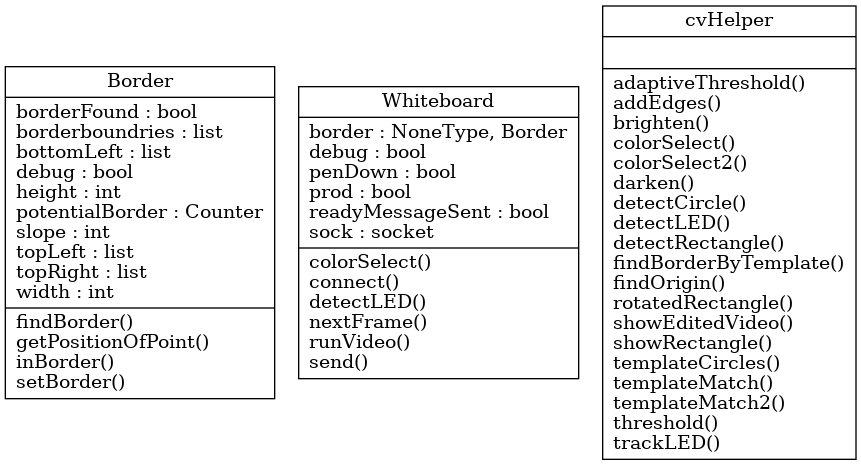
\includegraphics[scale=.5]{classes.png}
\end{figure}
\paragraph{} 
The main user interface is the whiteboard application that is projected onto a surface. 
The application allows users to draw on the surface using an IR LED as well as control the application. 
The control is available using the on screen buttons and allows the user to change the way the penstrokes are drawn. 
There are controls available to change the size and color of the pen. 
The user interface also displays a border for the image recognition to track where the user is drawing. 
Since this part of the application is stand alone and receives penstrokes from the image recognition processing via network stream.
Below is a mockup of what the user sees when the application first starts, they are able to draw anywhere within the border and use the buttons on the top left to control the pen type they are using. 
\begin{figure}[H]
\centering
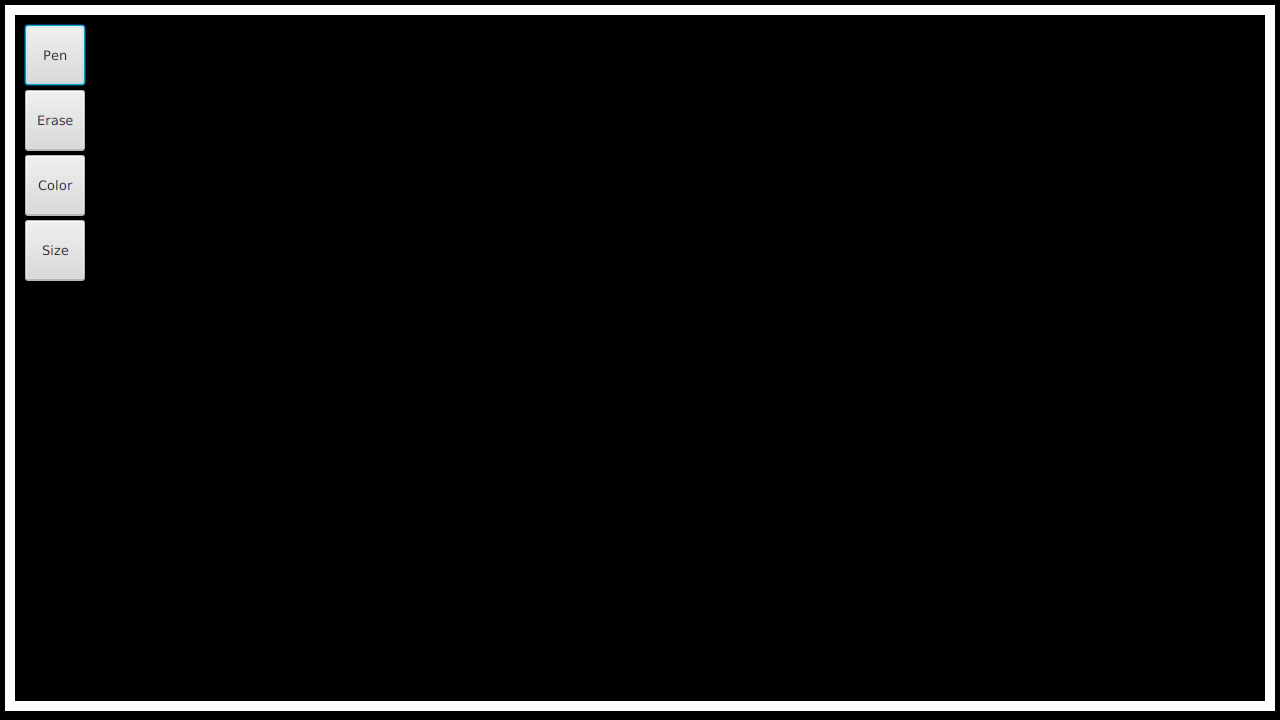
\includegraphics[scale=.25]{mockup.png}
\end{figure}

\section{Review Against Plan}
\paragraph{}
With the decision to make a computer process the video for image recognition instead of the Pi we must allocate some time to developing a method of streaming the video frames from the Pi over the network.
This was not planned originally since the video processing would happen on board rather than with an additional computer. 
In addition to video streaming we will likely have to put more time into networking than originally thought in order to make the application discoverable over the network and communicate between different parts of the application over the network. 

% \newpage \section{References} \printbibliography[heading=none]
\end{document}
